
The performance of the distributed algorithms are studied in this section by comparing with the centralized algorithms. The total number of queued packets after the current allocation and the total sum rate achieved by the network are used as the performance measures. Fig. \ref{fig-d-1} shows the performance of the algorithms for the system configuration represented by \me{\lbrace N,N_B,K,N_R \rbrace = \lbrace 3,2,8,1 \rbrace} with \me{N_T = 4} transmit antennas at each \ac{BS}. Each \ac{BS} serves \me{|\mc{U}_b| = 4} users in a coordinated manner to reduce the total number of backlogged packets at each \ac{BS}. Fig. \ref{fig-d-1.1} shows the total number of backlogged packets  and Fig. \ref{fig-d-1.2} plots the total rate achieved by different algorithms after each \ac{SCA} update. As pointed out in Section \ref{sec-4}, the performance and the convergence speed of the distributed algorithms are susceptible to the choice of the step size used in the subgradient update. Since the interference values are fixed for local subproblem in the primal approach, it may lead to infeasible solutions if the initial or any intermediate update using \eqref{primal-sg-update} is not valid.

The Fig. \ref{fig-d-1} plots the performance of the primal and the \ac{ADMM} solutions of the \ac{JSFRA} scheme using \ac{SCA} and by \ac{MSE} relaxation at each \ac{SCA} update points. In between the \ac{SCA} updates, the primal or the \ac{ADMM} schemes are performed for \me{J_{\max} = 20} iterations by exchanging either the fixed interference variables in the primal approach or the dual variables in the \ac{ADMM} scheme. It can be seen from Fig. \ref{fig-d-1} that the distributed algorithms approaches the centralized performance by exchanging minimal information between the coordinating \acp{BS}. The plot also includes the \ac{Q-WSRM} which performs similar to the other centralized schemes discussed in this paper.
\begin{figure*}
\centering
\begin{subfigure}{0.49\textwidth}
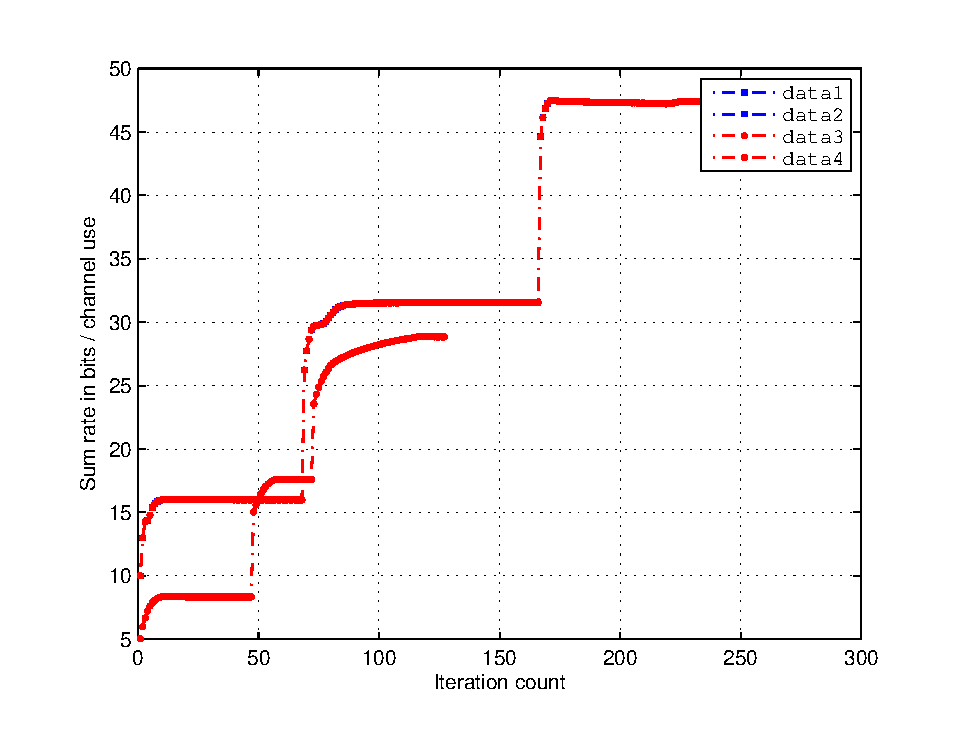
\includegraphics[width=\columnwidth]{fig-3}
\caption{Queue deviation}
\label{fig-d-1.1}
\end{subfigure}
\hfill
\begin{subfigure}{0.49\textwidth}
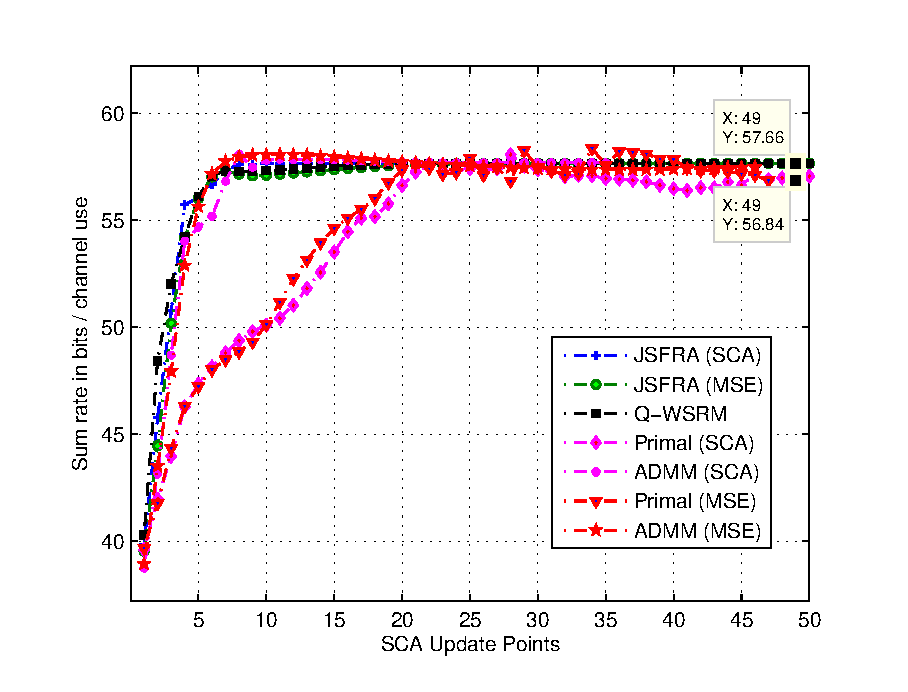
\includegraphics[width=\columnwidth]{fig-4}
\caption{Sum rate performance}
\label{fig-d-1.2}
\end{subfigure}
\caption[short]{Convergence plot for \me{\lbrace N,N_B,K,N_R \rbrace = \lbrace 3,2,8,1 \rbrace} model}
\label{fig-d-1}
\end{figure*}

In Fig. \ref{fig-d-2}, the performance of the distributed algorithms are studied for \me{K = 12} users utilizing \me{N = 6} sub-channels. The system considers \me{N_B = 3} \acp{BS}, each having \me{N_T = 4} transmit antennas serving \me{|\mc{U}_b| = 4} users equipped with \me{N_R = 2} antennas respectively. The users are assumed to be scattered over the cell boundary with the maximum interference power from any neighboring \ac{BS} follows \me{\mathbb{U}(0,-6)} dB. The performance of the algorithms are similar to the \me{N_B = 2} \ac{BS} scenario discussed earlier.

Fig. \ref{fig-d-2} plots the performance of the centralized and the distributed algorithms at each \ac{SCA} update. In case of the distributed algorithms, in between each \ac{SCA} update, the primal or the \ac{ADMM} exchanges are performed for \me{J_{\max} = 20} iterations. In practice, \me{J_{\max} = 1} can be set to perform the \ac{SCA} update, \ac{ADMM} or primal update, and the receive beamformer \me{\mvec{W}{k,n}} update at the same instant. The data tips are used to highlight the convergent points of various algorithms. The performance of the \ac{JSFRA} schemes using the primal decomposition are notably inferior compared to the \ac{ADMM} approach for the same schemes. It is mainly attributed to the difficulty in selecting the step size for the system employing \me{N_B \geq 3} \acp{BS}.
\begin{figure*}
\centering
\begin{subfigure}{0.49\textwidth}
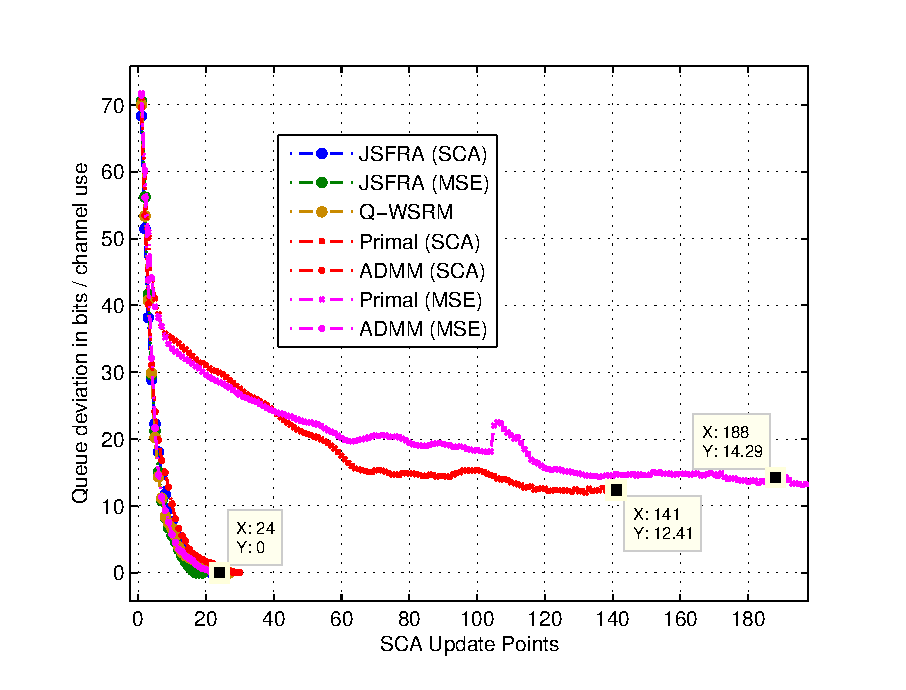
\includegraphics[width=\textwidth]{fig-5}
\caption{Queue deviation}
\end{subfigure}
\hfill
\begin{subfigure}{0.49\textwidth}
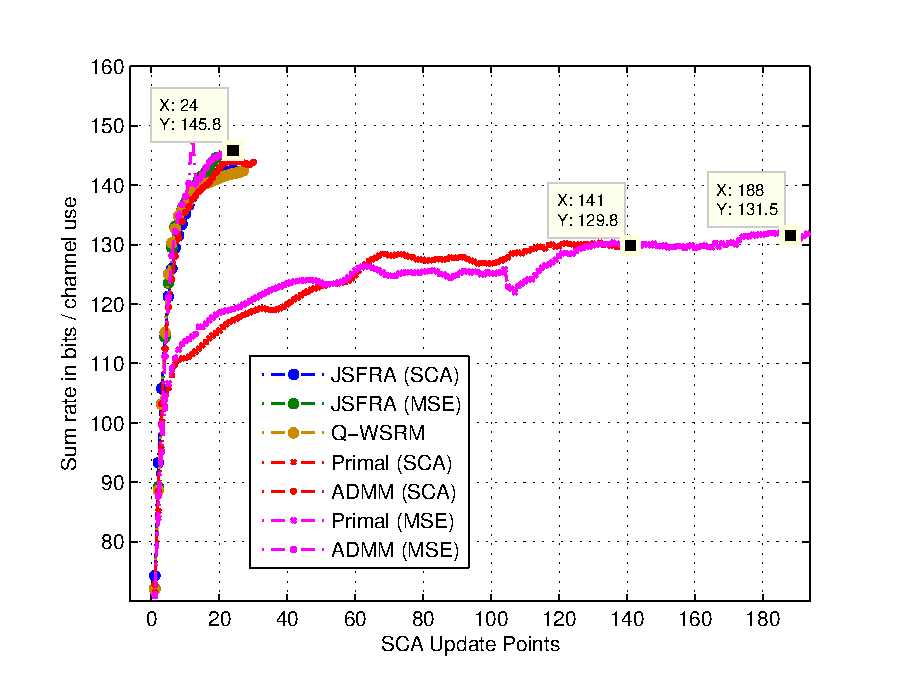
\includegraphics[width=\textwidth]{fig-6}
\caption{Sum rate performance}
\end{subfigure}
\caption{Convergence plot for \me{\lbrace N,N_B,K,N_R \rbrace = \lbrace 6,3,12,2 \rbrace} model}
\label{fig-d-2}
\end{figure*}

The performance of the \ac{MSE}-\ac{KKT} scheme discussed in Section \ref{sec-4.3} is presented in Fig. \ref{fig-d-3}. It compares the \ac{JSFRA} scheme with \me{\ell_1} and \me{\ell_2} norm cases in addition to the \ac{Q-WSRM} scheme. We compare the performance of the \ac{MSE}-\ac{KKT} scheme for the exponents \me{q=1} and \me{q=2}. The performance of the \me{\ell_1} \ac{JSFRA} scheme performs the best over other algorithms in minimizing the total number of queued bits after the current allocation due to its greedy approach. The inclusion of the additional second order rate term in \eqref{pf-1}, the \me{\ell_2} \ac{JSFRA} scheme achieves different performance than the \ac{Q-WSRM} scheme as shown in Fig. \ref{fig-d-3}. 

It can be seen from Fig. \ref{fig-d-3.2}, that the sum rate of the \me{q=1} \ac{KKT} approach outperforms other schemes in spite of Fig. \ref{fig-d-3.1} showing inferior queue minimizing performance. This due to the lack of the rate bounding constraint \eqref{kkt-mse-4.2}, which is simply given by \me{\sigma_{l,k,n}^{(i)} = \frac{a_k}{\log(2)}} providing no control for the excess allocations. For \me{q=2}, when the allocated rate exceeds the available queued bits, \me{\sigma_{l,k,n}^{(i)}} will be negative, thereby reducing \eqref{kkt-mse-4.1} as \me{\alpha_{l,k,n}^{(i)} < \alpha_{l,k,n}^{(i-1)}} to reduce the priority for the corresponding user in the next iteration. The performance of the closed form solution using the \ac{KKT} solution performs similar to the centralized schemes with \me{q=2} by limiting the rates beyond the available queued packets.
\begin{figure*}
\centering
\begin{subfigure}{0.49\textwidth}
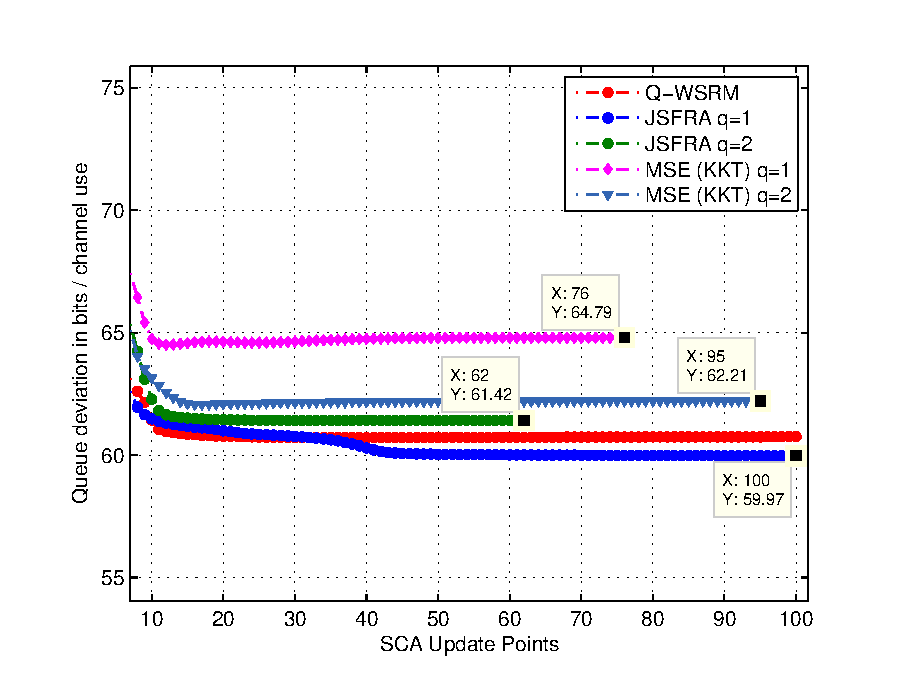
\includegraphics[width=\textwidth]{fig-9}
\caption{Queue deviation}
\label{fig-d-3.1}
\end{subfigure}
\hfill
\begin{subfigure}{0.49\textwidth}
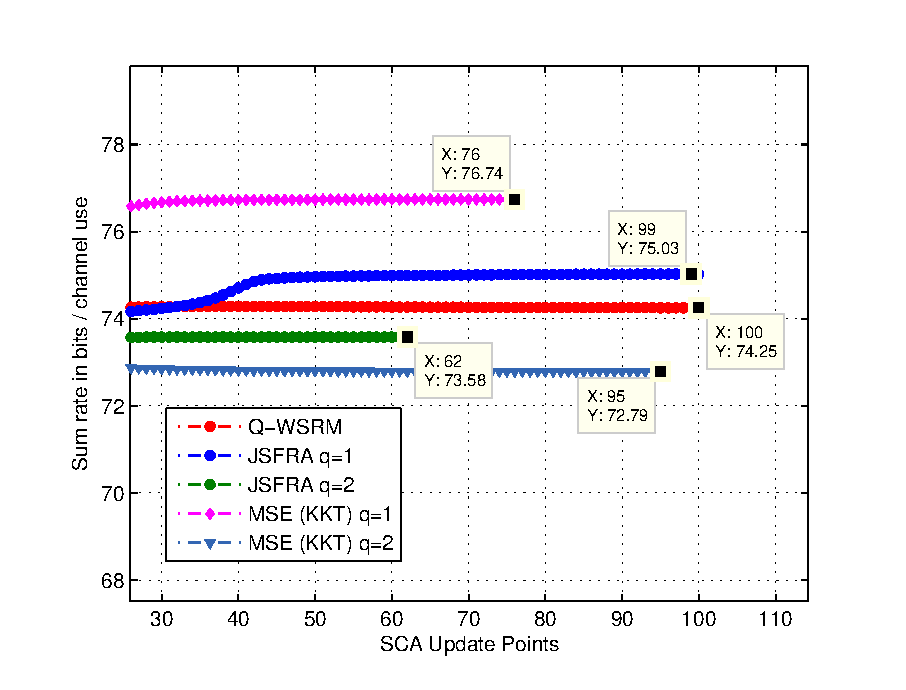
\includegraphics[width=\textwidth]{fig-10}
\caption{Sum rate performance}
\label{fig-d-3.2}
\end{subfigure}
%\caption{Convergence plot for \me{\lbrace N,N_B,K,N_R \rbrace = \lbrace 6,3,12,1 \rbrace} model}
%\caption{Convergence plot for \me{\lbrace N,N_B,K,N_R \rbrace = \lbrace 4,2,12,1 \rbrace} model}
\caption{Convergence plot for \me{\lbrace N,N_B,K,N_R \rbrace = \lbrace 4,2,12,1 \rbrace} model}
\label{fig-d-3}
\end{figure*}
